\subsection{Bitcoin}
% 
Created in 2009, Bitcoin is the first ever digital currency, that operates without a central authority in a completely decentralised manner. It is a cryptocurrency with largest market capitalisation\footnotemark and probably the most famous cryptocurrency worldwide.
% 
\footnotetext{Over USD 115 billion as of 01-04-2018. \url{https://coinmarketcap.com/}, accessed 01-04-2018
}
% 
Bitcoin was proposed by a person or a group under the pseudonym Satoshi Nakamoto, whose identity is not known to date~\cite{Feins2017SatoshiBitcoin}. The initial proposal consisted of a white-paper describing the system~\cite{NakamotoBitcoin:System} and the reference implementation written in  C++ \footnotemark.
% 
\footnotetext{Original repository has been moved from SourceForge and can now be found on Github. \url{https://github.com/bitcoin/bitcoin/tree/4405b78d6059e536c36974088a8ed4d9f0f29898}, accessed 01-04-2018}

In the white-paper, Nakamoto proposes a decentralised currency, based on a proof-of-work blockchain. The blockchain is made up of blocks, where each block comprises a different set of transactions~\cite{Decker2013InformationNetwork, Judmayer2017BlocksMechanisms}.

\subsubsection{Proof of work}
To include a new block in the blockchain, certain amount of work needs to be carried out by the node. This is a protection against the attempts to include counterfeit data in the blockchain. As discussed earlier, to falsify a past block, an attacker would need to recalculate all the subsequent blocks. Furthermore, they would need to provide proof-of-work for all the subsequent blocks. Since the \acrfull{pow} is computationally intensive, it would be practically impossible for the attacker to outpace the honest nodes~\cite{NakamotoBitcoin:System}.

In case of Bitcoin, the proof-of-work consists of finding such a hash value, that is below a given constant -- \textit{target}. In Bitcoin, this hash value is computed over the hash value of previous block, timestamp\footnotemark, root hash of the transactions\footnote{Transactions are ordered in a Merkle tree.} and a random number, called \textit{nonce}. The work of the nodes consists of generating a new nonce and computing a new hash. If value of this hash is smaller than the target, a valid block is produced and can be broadcasted to the other nodes. Figure~\ref{fig:blocks-bitcoin} shows the composition of the block in detail. By design, a new block should be mined approximately every 10 minutes. The network automatically adjusts the value of the target to meet this requirement (if the value of the target remained the same, increasing speed of computers would result in faster block production speed over time)~\cite{Decker2013InformationNetwork}.
% 
\footnotetext{The timestamp is a local UNIX time of the node. However, this timestamp does not to be very accurate (approximate allowed accuracy is $\pm$ 1 hour). It can happen, that the timestamps in blocks are not in order. The goal of the timestamp is to increase the difficulty of forging the blocks. \url{https://en.bitcoin.it/wiki/Block_timestamp}, accessed 01-04-2018}
% 
\begin{figure}[ht]
    \centering
    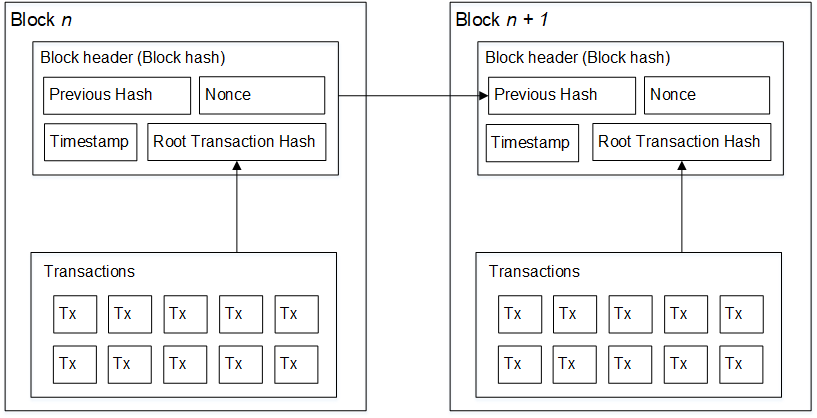
\includegraphics[width=.95\textwidth]{blocks-bitcoin}
    \caption{Composition of the Bitcoin blockchain. Work of a node consists of repeatedly hashing the block header, trying out different nonce every time.}
    \label{fig:blocks-bitcoin}
\end{figure}
% 
\subsubsection{Network of nodes}
Each node carries out work at its own pace, trying different values for nonce and hashing the block header. Essentially, this is simply trying to use the brute force to produce a hash below a threshold. This process is also referred to as \textit{mining}. Once the hash is below the current threshold, a new block is mined. The new block is then broadcasted to all the nodes connected to the network~\cite{NakamotoBitcoin:System}. When a node receives a block it has not seen before, it first verifies the transactions in the block and then introduces it to its peers. The average time for a block to reach the whole network is 12.6 seconds~\cite{Decker2013InformationNetwork}. It is well below the block generation speed (1 block approximately every 10 minutes), however, it is not crucial for the network that every node has a copy of the latest block: ``\textit{If a node does not receive a block, it will request it when it receives the next block and realises it missed one.}''~\cite{NakamotoBitcoin:System}.
% 
\subsubsection{Transactions and accounts}
A Bitcoin transaction is the act of moving the funds from one account to another~\cite{Judmayer2017BlocksMechanisms}, as illustrated in Figure~\ref{fig:bitcoin-tx}. We explain this process, we must first define the notion of an account.

\begin{figure}[ht]
    \centering
    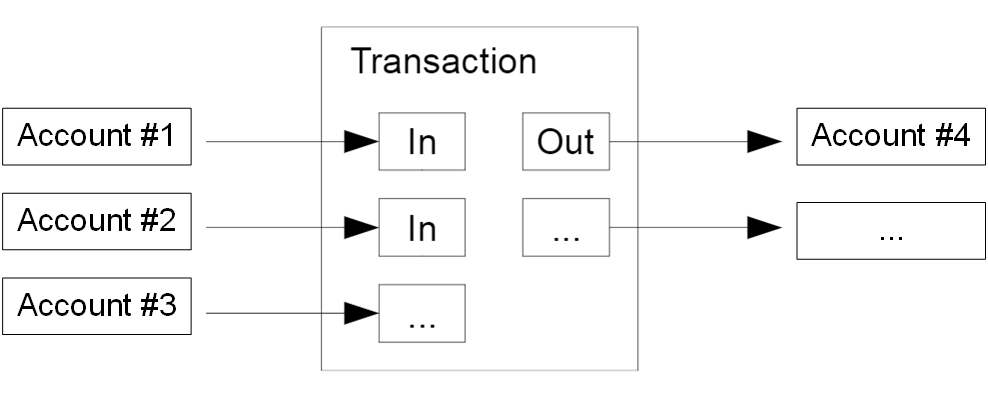
\includegraphics[width=\textwidth]{bitcoin-tx}
    \caption{A Bitcoin transaction representation. Each transaction has to have at least one input and one output. The inputs and outputs can have various values, but the total sum of the inputs needs to be equal to or greater than the number of outputs. The only exemption from this rule is the reward for the miner that found a new block. Such transaction only has outputs and no inputs. Taken from~\cite{NakamotoBitcoin:System}, edited.}
    \label{fig:bitcoin-tx}
\end{figure}

An account is pair of a public and private key. Bitcoin uses the \acrfull{ecdsa} for the key pair generation~\cite{Decker2013InformationNetwork}. The account is identified by its public address. The public address is generated from the public key through a series of hashes. Figure~\ref{fig:public-address-gen} describes this process in further detail.
% 
\begin{figure}[p]
    \centering
    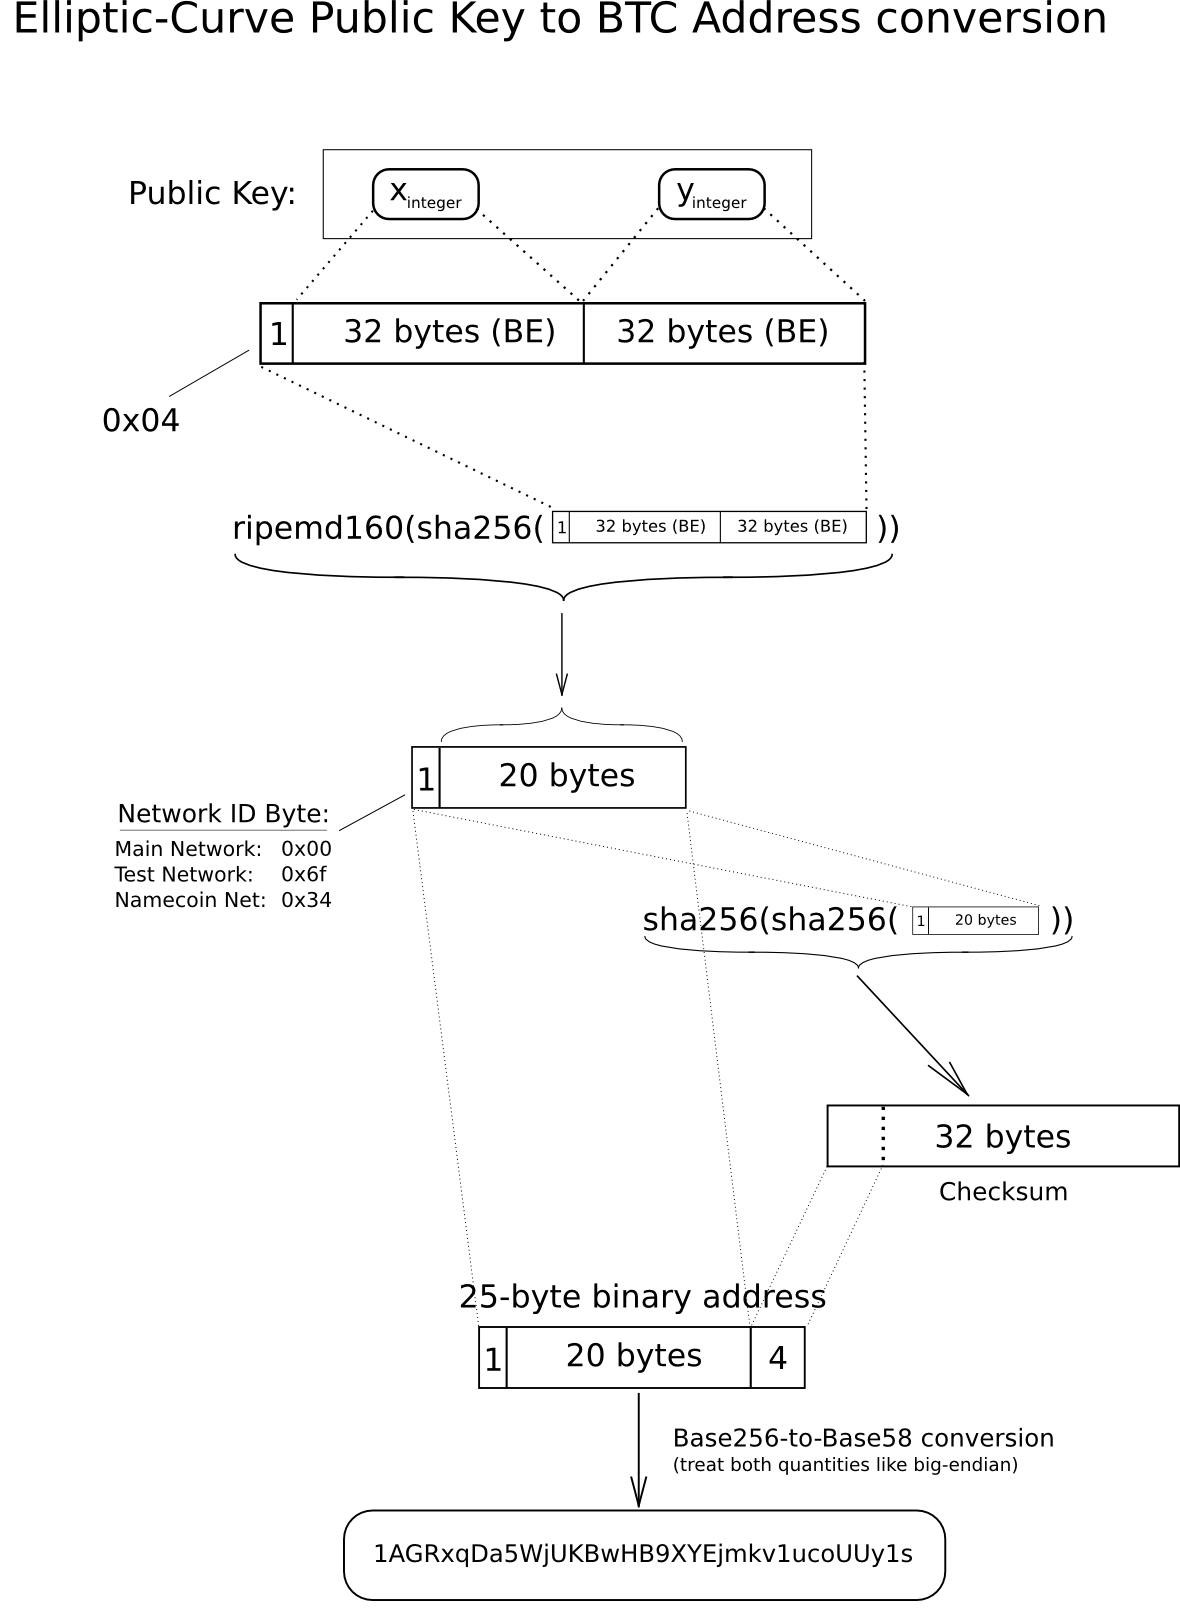
\includegraphics[height=.85\textheight]{PubKeyToAddr}
    \caption{First, a public key and a prefix are hashed using SHA-256 and then RIPEMD-160. This value is hashed twice with SHA-256 to generate a checksum. The result is composed of 1 network byte, RIPEMD-160 hash and first 4 bytes of checksum.}
    \label{fig:public-address-gen}
\end{figure}

A transaction contains a number of inputs and a number of outputs. The sum of inputs must be equal or greater than the sum of the outputs~\cite[p. 27]{Judmayer2017BlocksMechanisms}. In case the sum of the inputs of the transaction is greater than sum of the outputs, the excess is collected by the miner as the \textit{transaction fee}.

Every unit of the currency has a history of transactions up to its origin. This chain of ownership verifies the validity of that particular unit and serves as a proof, that the unit is not counterfeit. Transferring funds from one account to another comprises hashing the public address of the future owner and hash of the last transaction. The resulting hash is then singed with the private key of the previous owner~\cite{NakamotoBitcoin:System}, as illustrated in Figure~\ref{fig:chain-ownership}. Once the transaction is signed, it is distributed to the network and can be included in a block.
% 
\begin{figure}[ht]
    \centering
    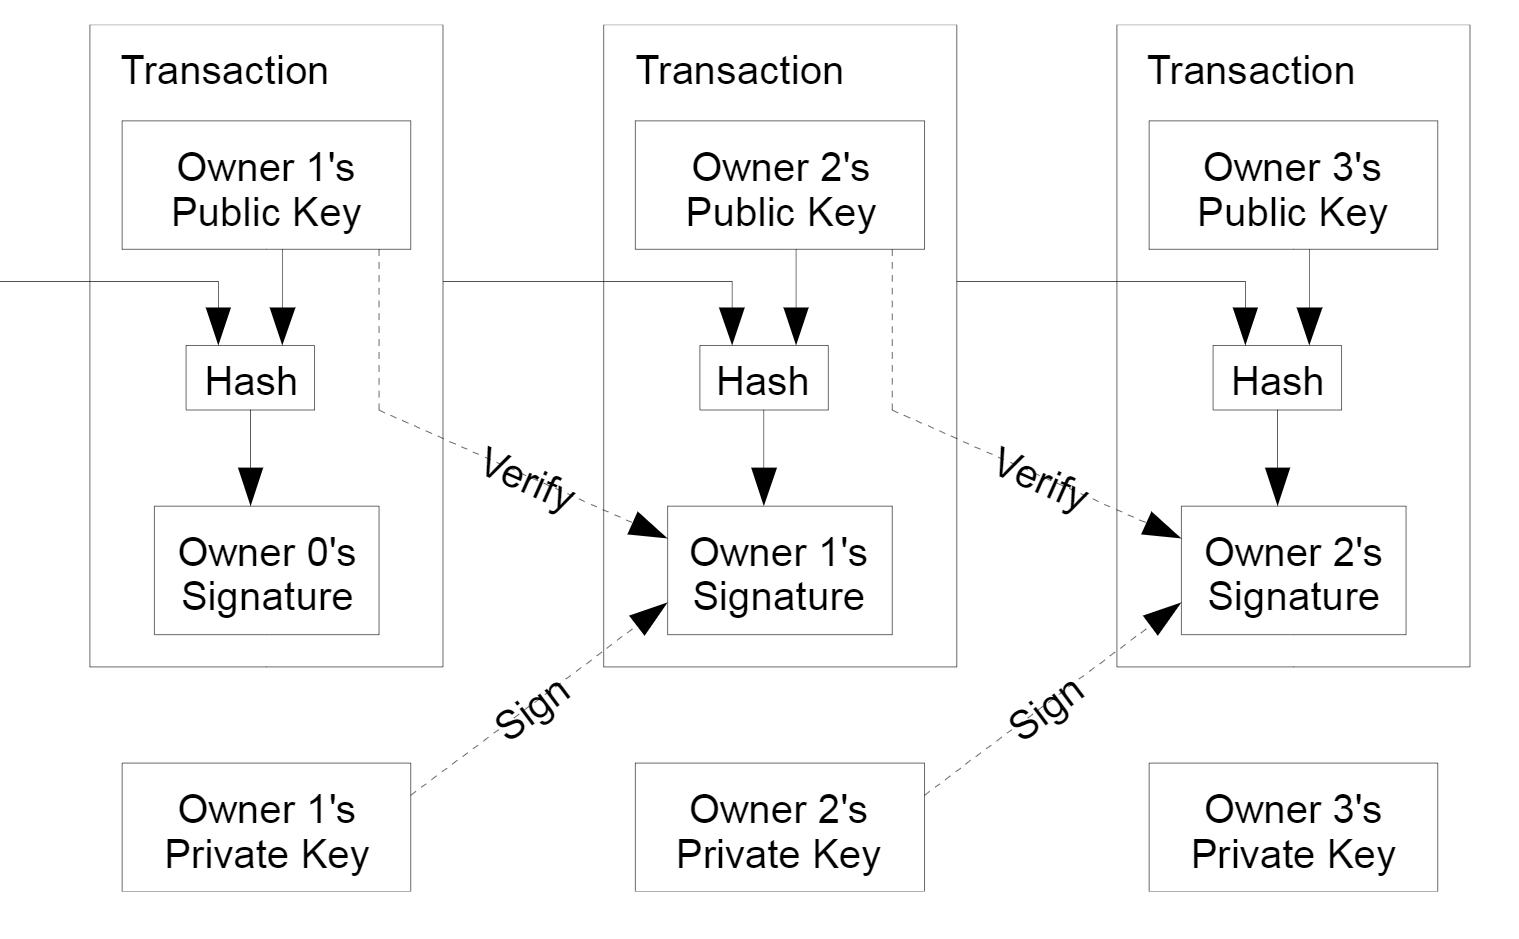
\includegraphics[width=.95\textwidth]{chain-ownership}
    \caption{Chain of ownership for unit of currency. Taken from~\cite{NakamotoBitcoin:System}.}
    \label{fig:chain-ownership}
\end{figure}

\subsubsection{Value}
Besides the system described above, the term `Bitcoin' also refers to a basic \textit{unit} of the currency. Bitcoin is further divisible into smaller units. The smallest unit is 1~satoshi. 1~Bitcoin contains 100~000~000~satoshi. 1~Bitcoin at the time of writing has a value of EUR~5~666. The value of Bitcoin is very volatile and has increased and decreased by tens or percents, sometimes even within hours~\cite{Adkisson2018WhyVolatile}. The peak in the value of Bitcoin has occurred on December~16,~2017 when 1 Bitcoin was traded for around EUR~16~500.

\subsubsection{Incentives}
Node that successfully mined a block, collects fees from all the included transactions, which poses as an incentive for the nodes to stay honest and keep mining new blocks. In addition to the transaction fees, there is a reward associated with each newly mined block. This reward at the time of writing is 12.5 coins and halves every 210~000 blocks~\cite{Judmayer2017BlocksMechanisms}, with expected decrease again in 2020. The reward is a transaction with no inputs and is the only exception, where the outputs of a transactions are higher than its inputs. The reward for mining a block will decrease to zero approximately in 2140. The supply of the currency is therefore limited and there is an upper bound to the number of Bitcoins that will ever exist\footnotemark.

\footnotetext{As~\cite[p. 38]{Judmayer2017BlocksMechanisms} notes, this limit is only ensured pragmatically and is only valid if majority of the network observes this rule.}

\subsubsection{Altcoins}
The Bitcoin proposal and the first reference client were both published publicly. Not only this allowed for easy adoption within the community, it also enabled creation of cryptocurrencies derived from Bitcoin. These cryptocurrencies, that build on top of Bitcoin and only change few aspects of the system are known as \textit{altcoins}~\cite{Judmayer2017BlocksMechanisms}. Some of these currencies gained exchange value and are still in use by the general public. Others may be targeted on a specific use-case or are only used by narrow communities. Furthermore, some of these altcoins can also serve as proof-of-concept for any improvement proposals for the Bitcoin network~\cite{Tarasiewicz2015ChapterExperiments}. Litecoin, Dogecoin, Namecoin and Talkcoin\footnotemark are only few of the many examples of altcoins. Their differences from Bitcoin and their uses are shown in Table~\ref{tab:altcoins}.
% 
\footnotetext{\url{https://litecoin.org/}\\
\url{https://dogechain.info/}\\
\url{https://namecoin.org/}\\
\url{https://bitcointalk.org/index.php?topic=781207/} all accessed 18-05-2018}
% 
\begin{table}[ht]
    \centering
    \begin{tabularx}{\textwidth}{|l|X|m{10em}|}
         \hline
         \textbf{Name}&\textbf{Main difference from Bitcoin}&\textbf{Use}\\
         \hline
         \hline
         Litecoin&Shorter block time, different \acrshort{pow} algorithm&Value exchange\\
         \hline
         Dogecoin&Shorter block time&Humorous\\
         \hline
         Namecoin&Possible distributed data storage&Domain name registration (.bit), various other uses\\
         \hline
         Talkcoin&Possible message exchange between users, faster block time&Chatting\\
         \hline 
    \end{tabularx}
    \caption{Comparison of selected altcoins.}
    \label{tab:altcoins}
\end{table}